\setbeamercolor{background canvas}{bg=fitblue}
\begin{frame}
\frametitle{Shadows / Stíny}
\begin{center}
\Huge {\color{white}Shadows / Stíny}
\end{center}
\end{frame}
\setbeamercolor{background canvas}{bg=white}

\begin{frame}\frametitle{Why do we need shadows? / Proč potřebujeme stíny?}
  \begin{figure}[h]
    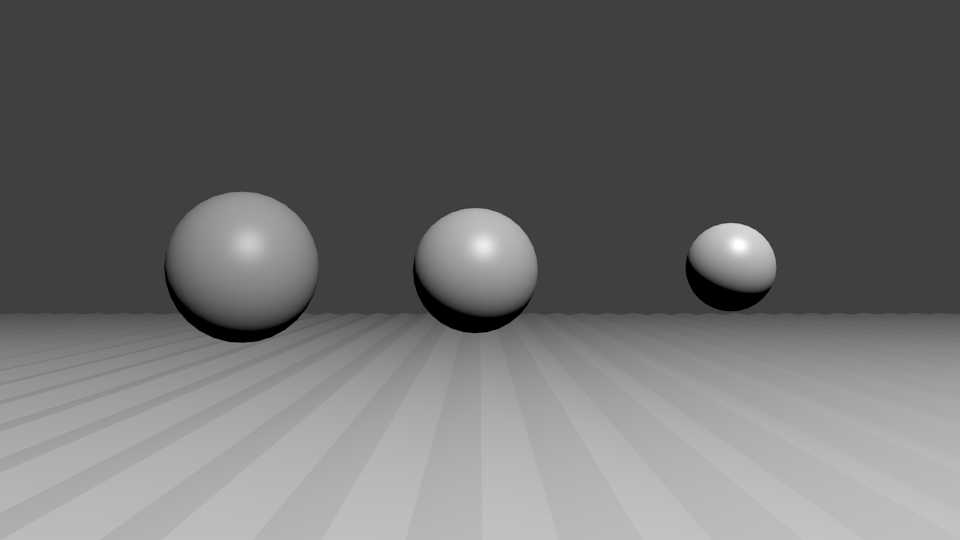
\includegraphics[width=11.5cm,keepaspectratio]{pics/shadows/whyShadows/noShadows}
  \end{figure}
\end{frame}

\begin{frame}\frametitle{Why do we need shadows? / Proč potřebujeme stíny?}
  \begin{figure}[h]
    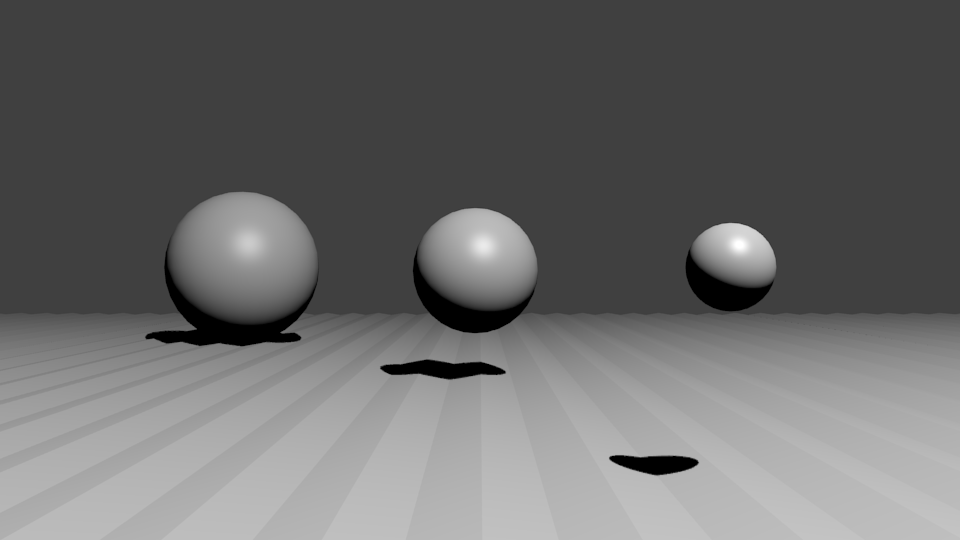
\includegraphics[width=11.5cm,keepaspectratio]{pics/shadows/whyShadows/shadows}
  \end{figure}
\end{frame}

\begin{frame}\frametitle{Why do we need shadows? / Proč potřebujeme stíny?}
  \begin{figure}[h]
    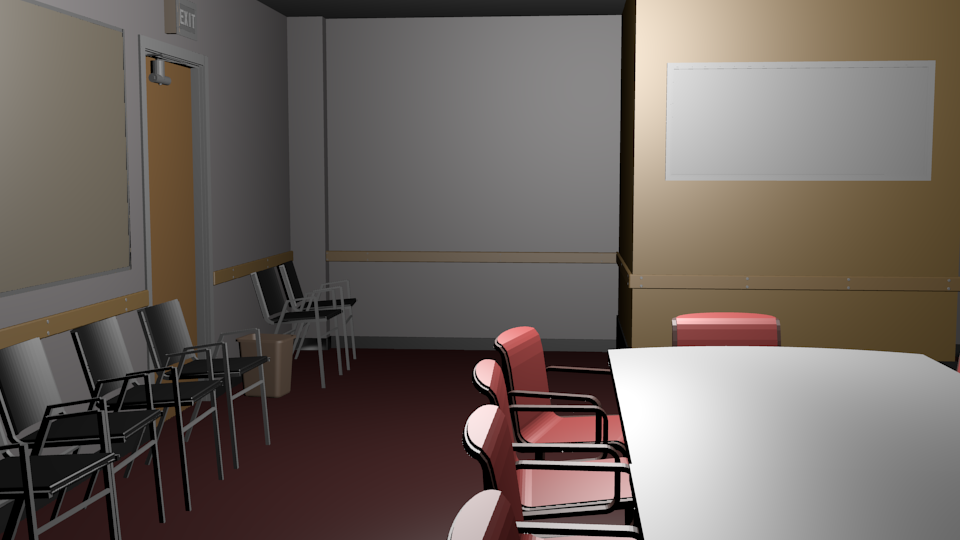
\includegraphics[width=11.5cm,keepaspectratio]{pics/shadows/whyShadows/conferenceNoShadows}
  \end{figure}
\end{frame}

\begin{frame}\frametitle{Why do we need shadows? / Proč potřebujeme stíny?}\scriptsize
  \begin{itemize}
    \item Shadows help us to comprehend 3D structure of a scene.
    \item Mutual location of objects.
  \end{itemize}
  \begin{itemize}
    \item Stíny pomáhají pochopit 3D scénu.
    \item Vzájemné polohy mezi objekty.
  \end{itemize}
  \begin{figure}[h]
    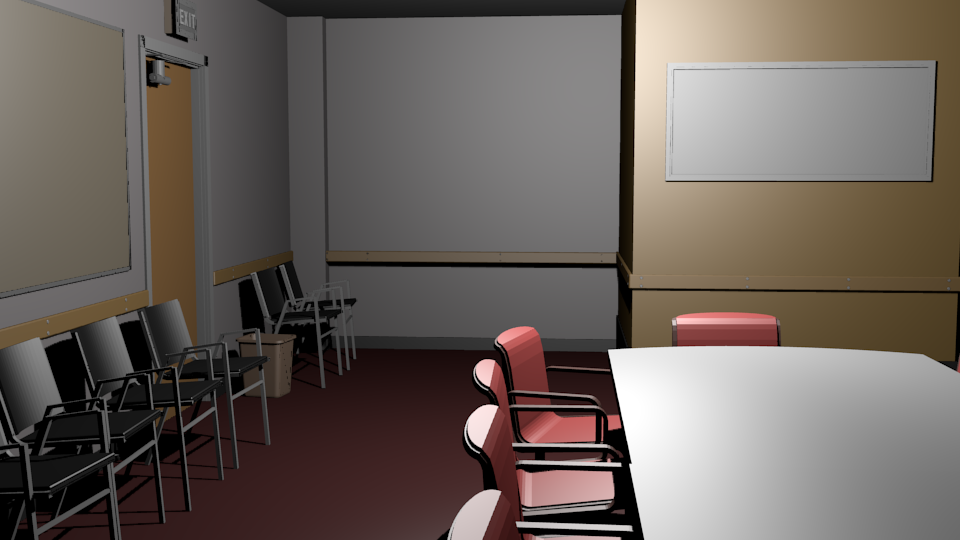
\includegraphics[width=11.5cm,keepaspectratio]{pics/shadows/whyShadows/conferenceShadows}
  \end{figure}
\end{frame}

\begin{frame}\frametitle{Types of light sources / Druhy světel}
  \begin{itemize}
    \item Omnidirectional point light source.
    \item Spot light source.
    \item Directional light source.
  \end{itemize}
  \begin{figure}[h]
    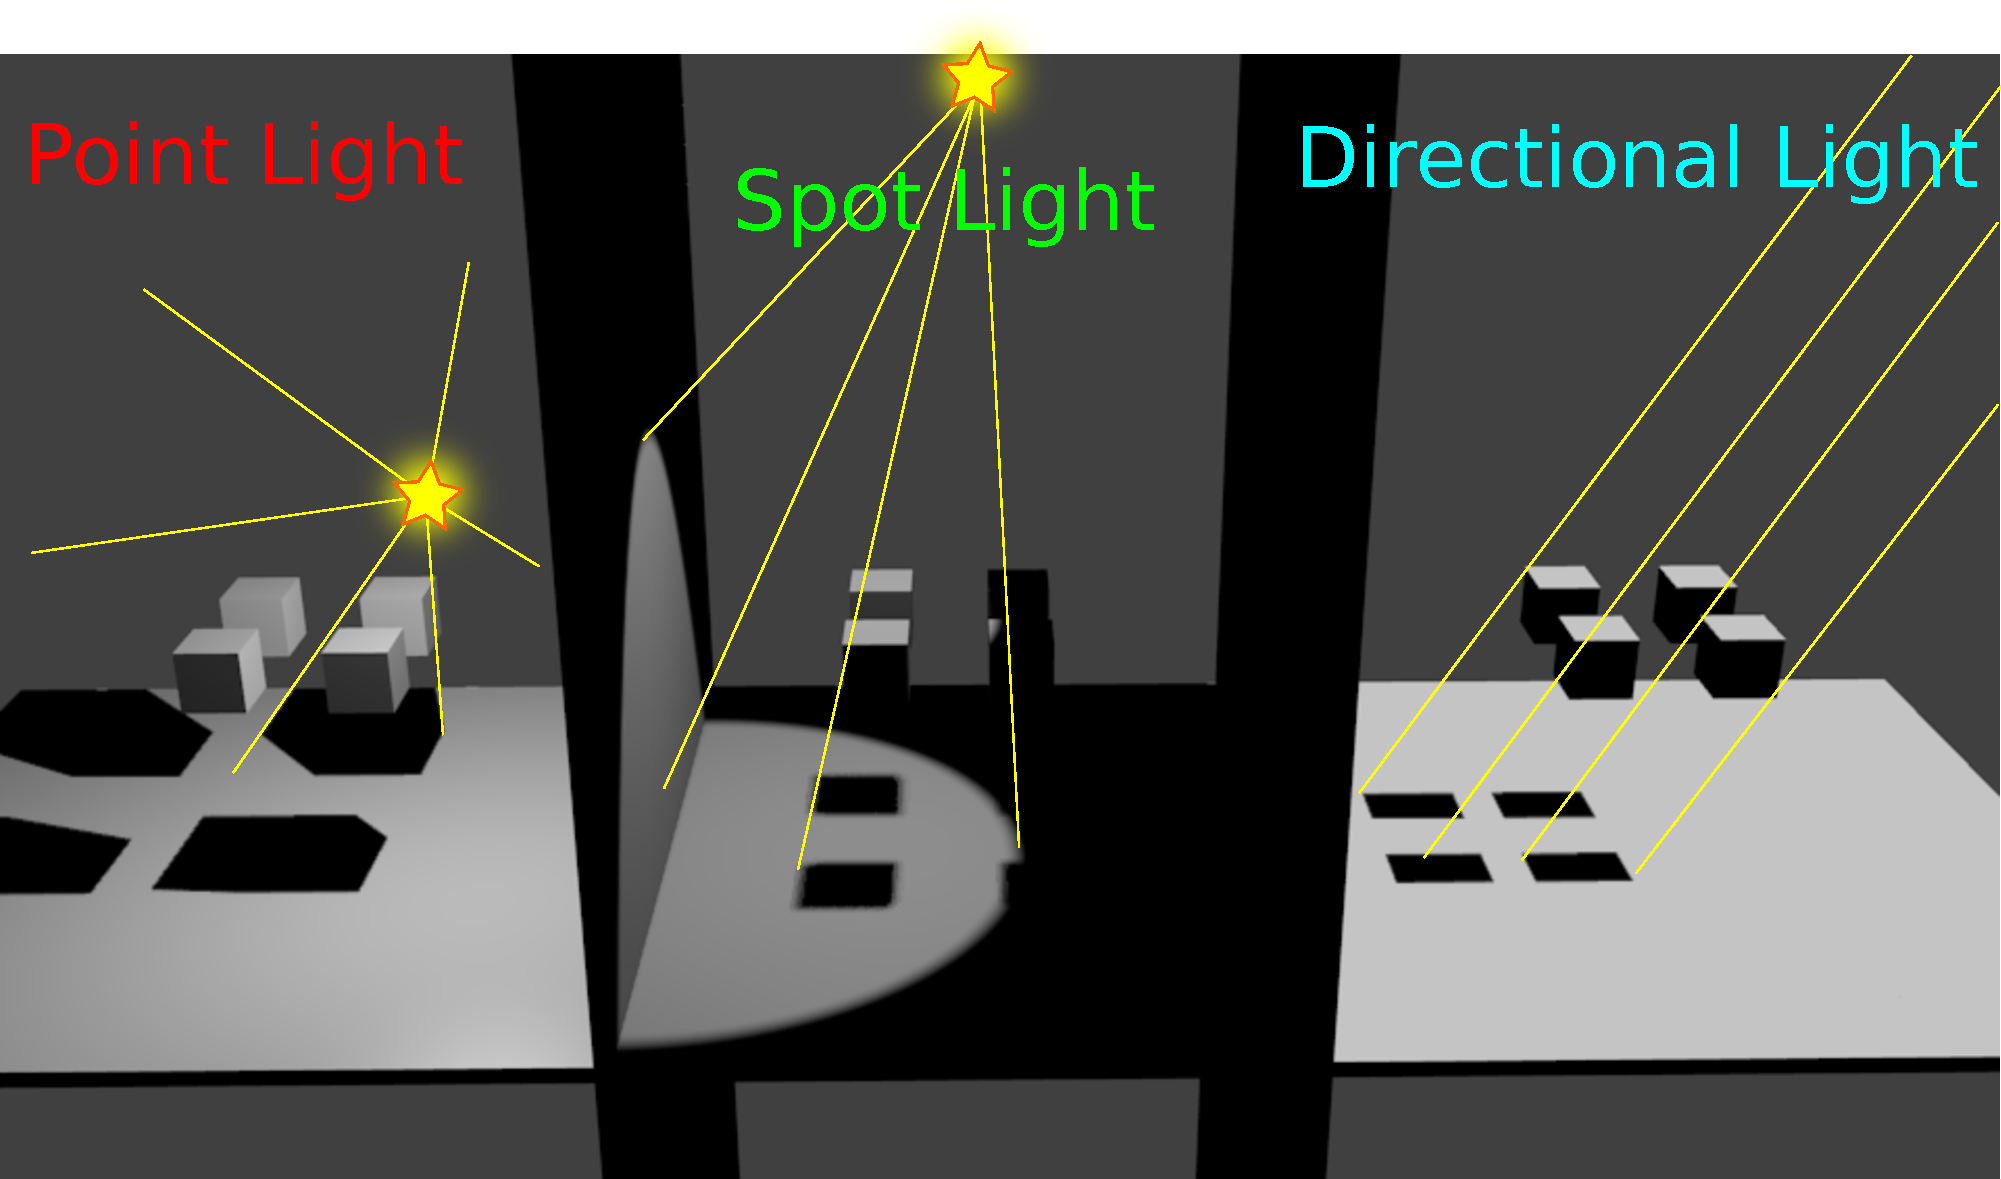
\includegraphics[width=10.5cm,keepaspectratio]{pics/shadows/lightTypes/lightTypes.pdf}
  \end{figure}
\end{frame}

\begin{frame}\frametitle{Types of shadows / Druhy stínů}\scriptsize
  \begin{itemize}
    \item Hard shadows are created by infinitesimal light sources (common in computer graphics).
    \item Soft shadow are created from area light sources.
  \end{itemize}
  \begin{itemize}
    \item Tvrdé stíný vznikají z nekonečně malých světelných zdrojů (časté v počítačové grafice).
    \item Měkké stíny vznikají z plošných zdrojů světla.
  \end{itemize}
  \begin{figure}[h]
    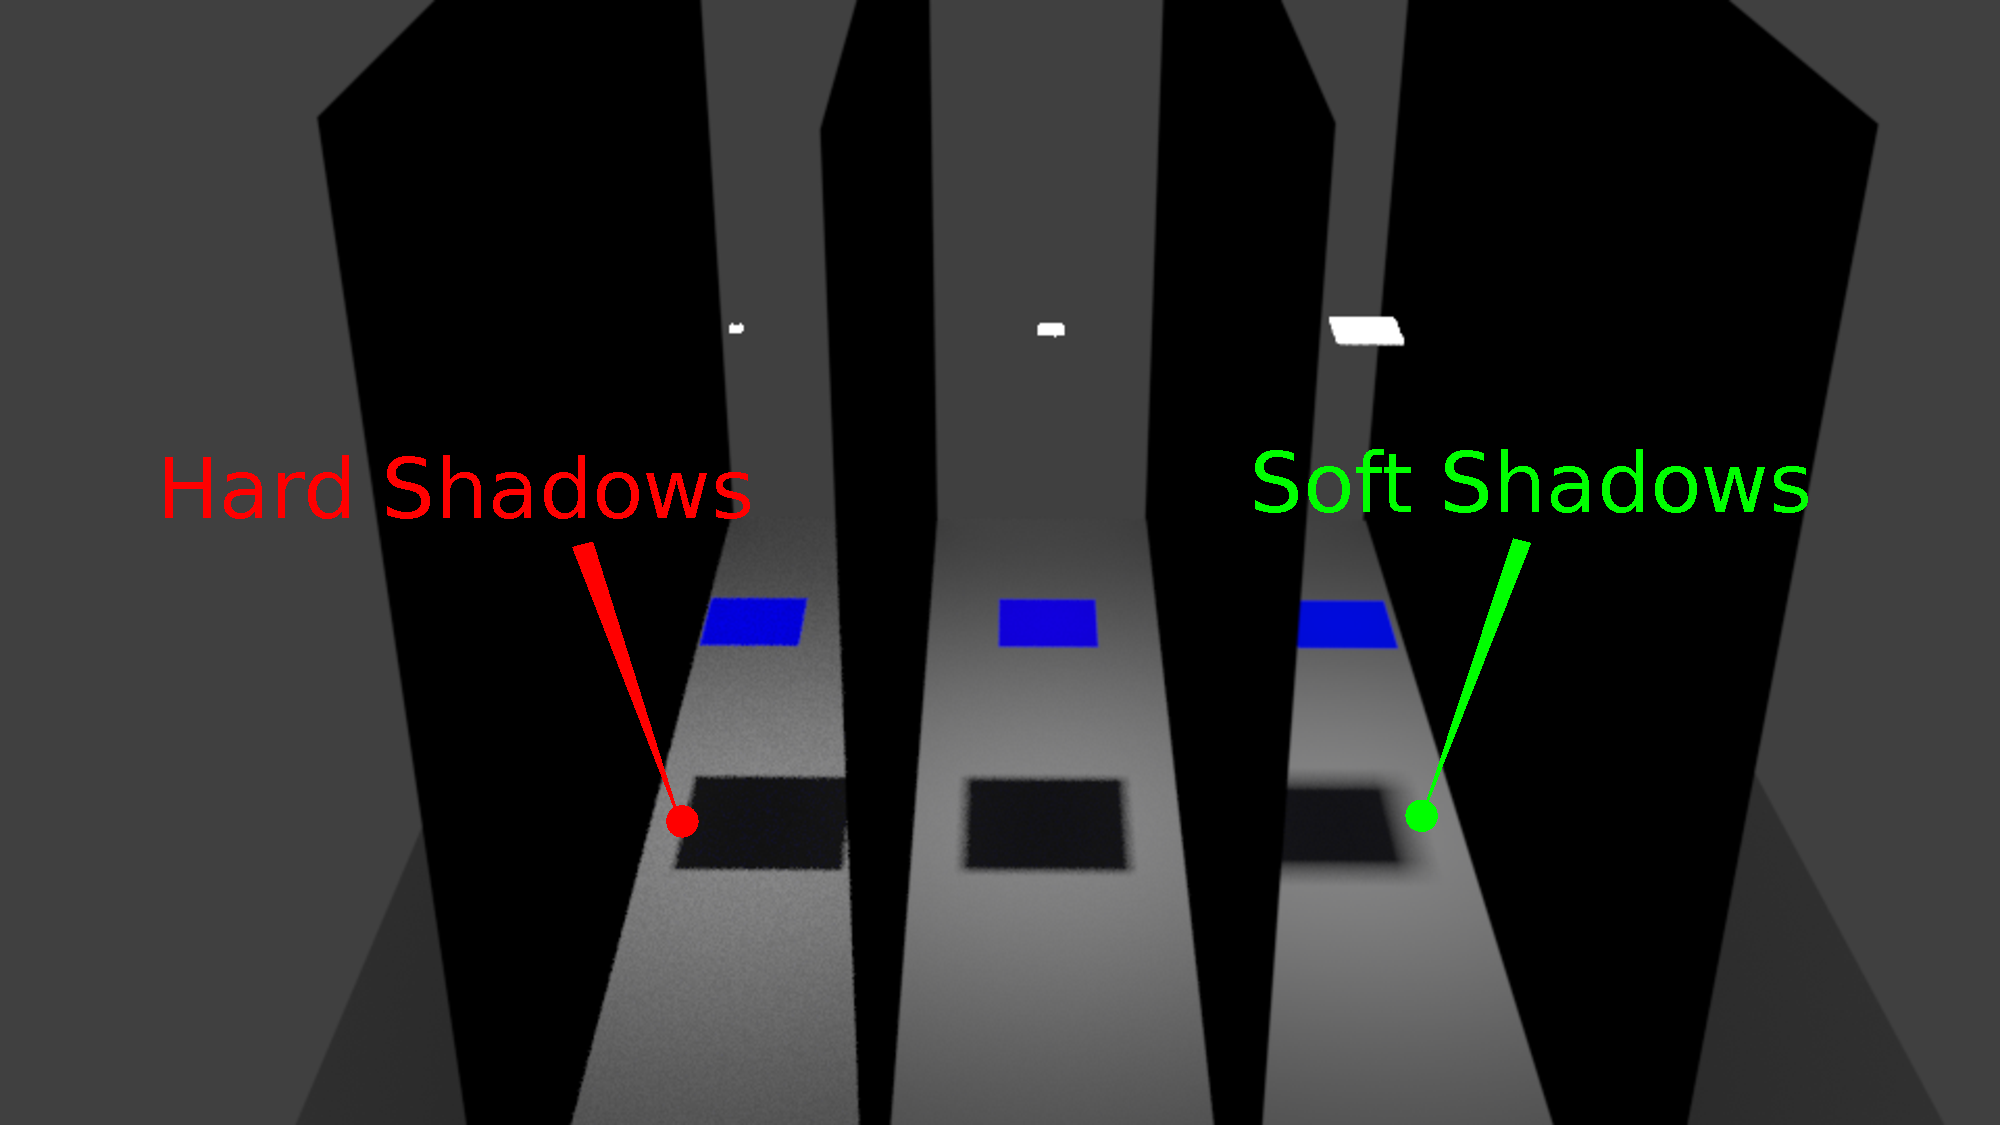
\includegraphics[width=11cm,keepaspectratio]{pics/shadows/hardShadow/hardShadow.pdf}
  \end{figure}
\end{frame}

\begin{frame}\frametitle{Types of shadows / Druhy stínů}\scriptsize
  \begin{itemize}
    \item Fully lit parts of the scene see all points of the light source.
    \item Fully shadowed parts of the scene do not see any point of the light source.
    \item Half shadow (penumbra) is created in regions with partial visibility to the light source.
  \end{itemize}
  \begin{figure}[h]
    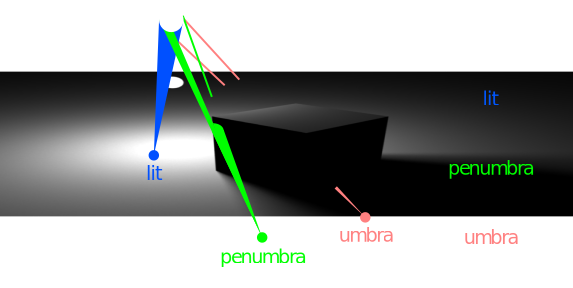
\includegraphics[width=11cm,keepaspectratio]{pics/shadows/penumbra/penumbra}
  \end{figure}
\end{frame}

\begin{frame}\frametitle{Types of shadows / Druhy stínů}\scriptsize
  \begin{itemize}
    \item Shadows are created from direct illumination (can be hard, if the light source is small).
    \item Shadows are created from indirect illumination (soft shadows).
  \end{itemize}
  \begin{itemize}
    \item Stíny vznikají z přímého osvětlení (můžou být tvrdé, pokud je světlo malé).
    \item Stíny vznikají z nepřímého osvětlení (měkké stíny).
  \end{itemize}
  \begin{figure}[h]
    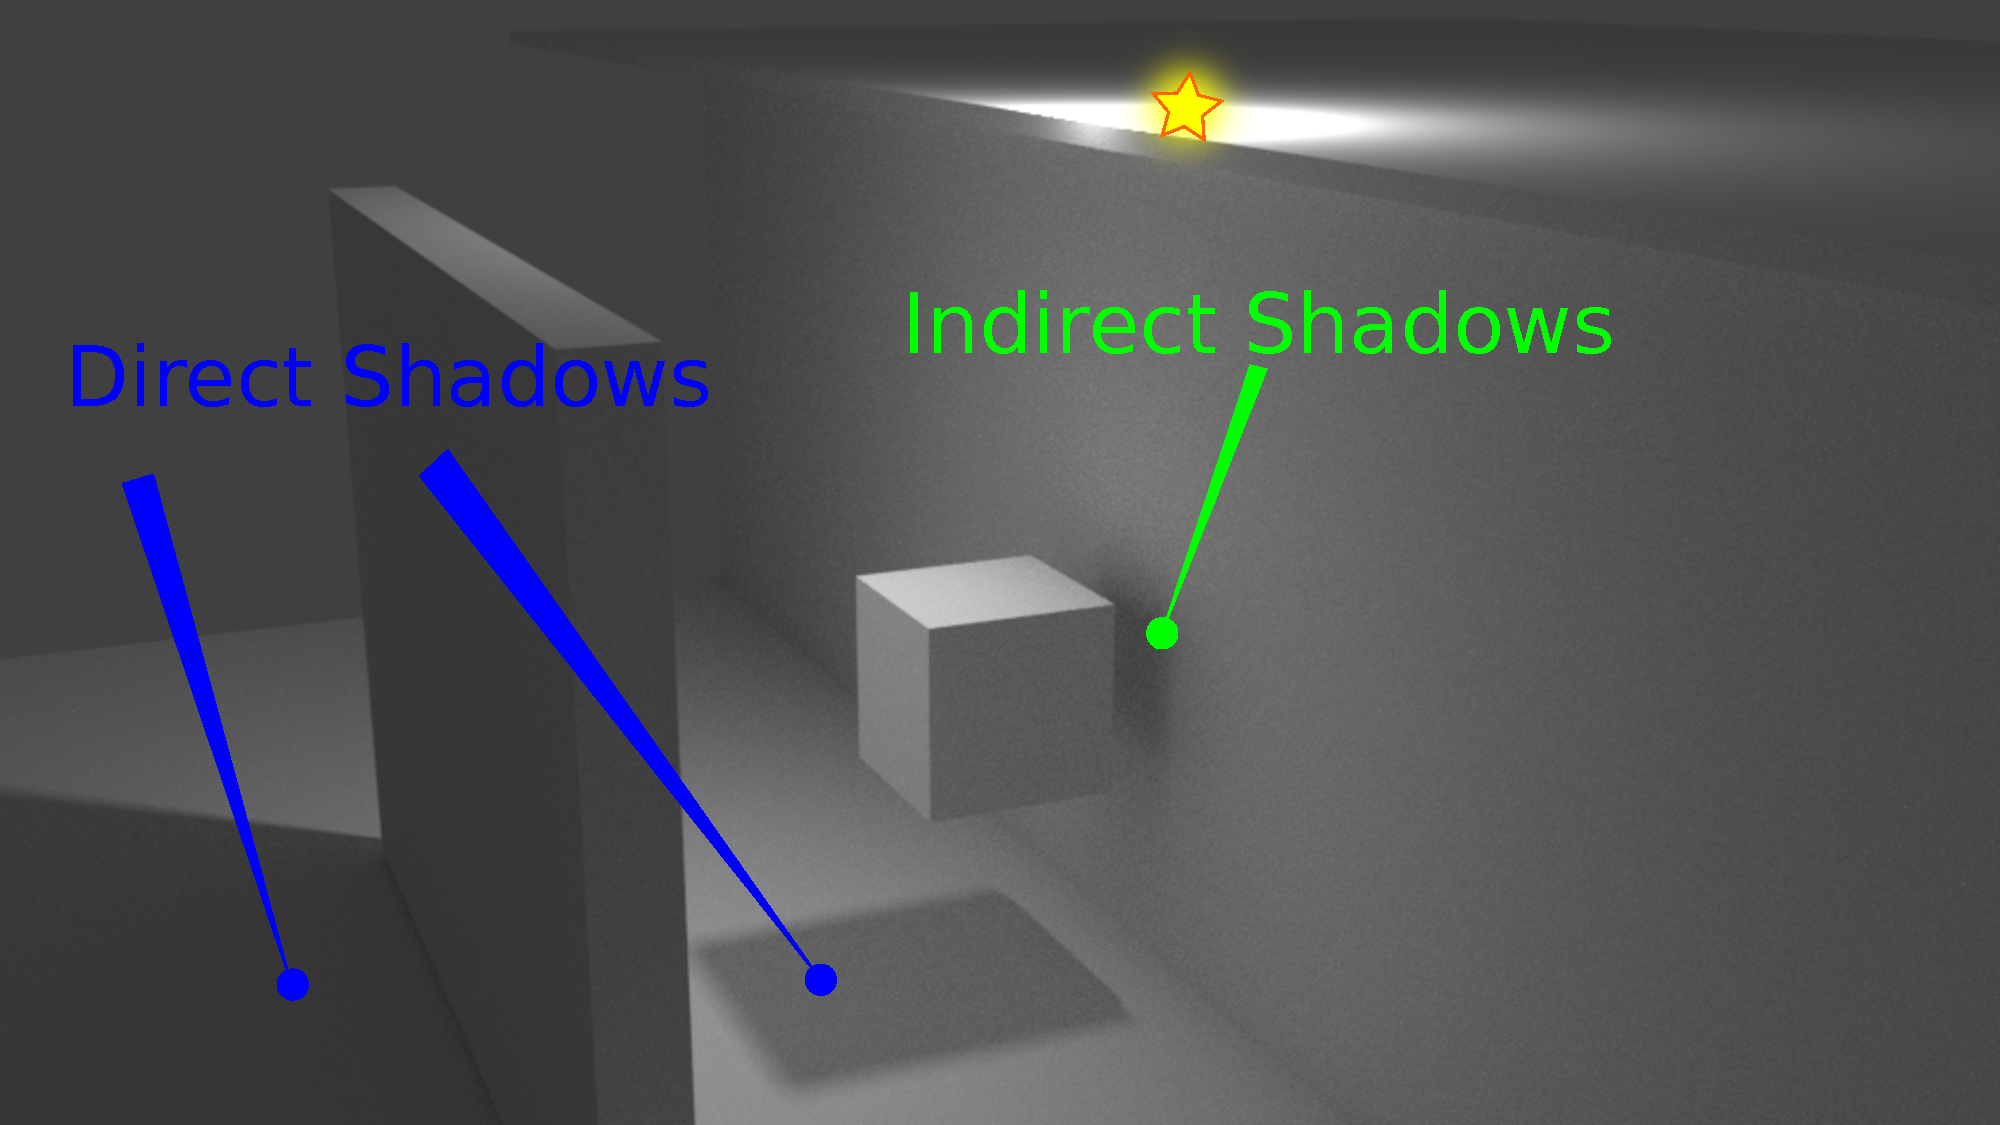
\includegraphics[width=11cm,keepaspectratio]{pics/shadows/indirectShadow/indirectShadows.pdf}
  \end{figure}
\end{frame}

\begin{frame}\frametitle{Ambient occlusion}
  \begin{itemize}
    \item Ambient occlusion - approximation of global illumination.
    \item Ambient occlusion - metoda pro aproximaci části globálního osvětlení a simulaci stínů nepřímého osvětlení.
  \end{itemize}
  \begin{figure}[h]
    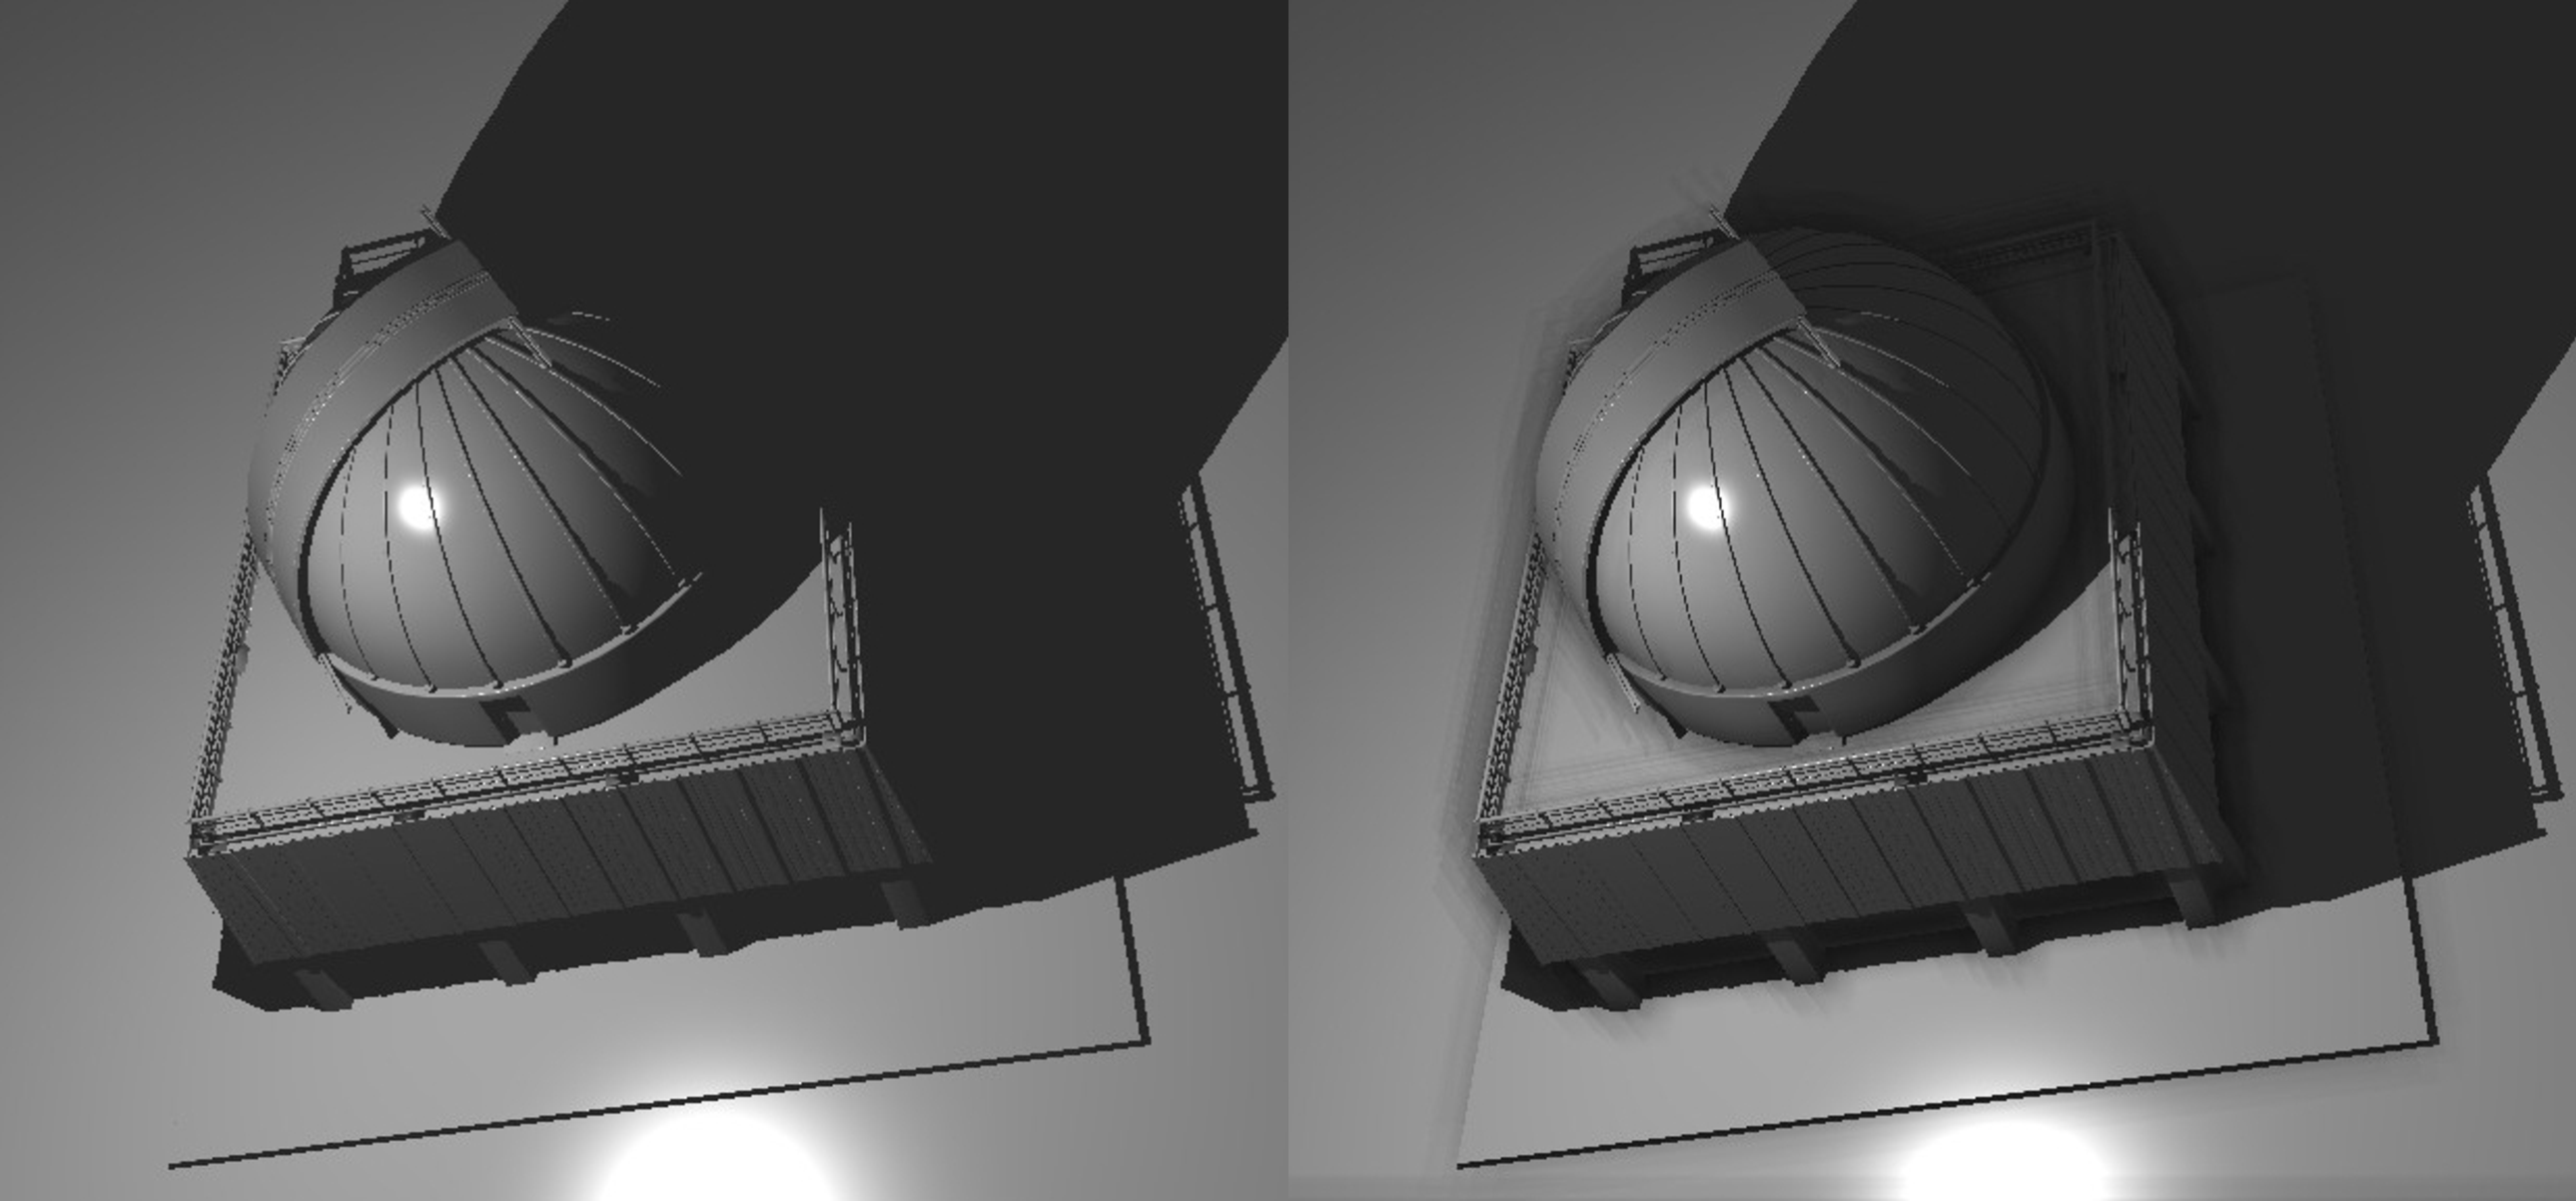
\includegraphics[width=11.5cm,keepaspectratio]{pics/shadows/ambientOcclusion/difference}
  \end{figure}
\end{frame}

\begin{frame}\frametitle{Ambient occlusion}
  \begin{figure}[h]
    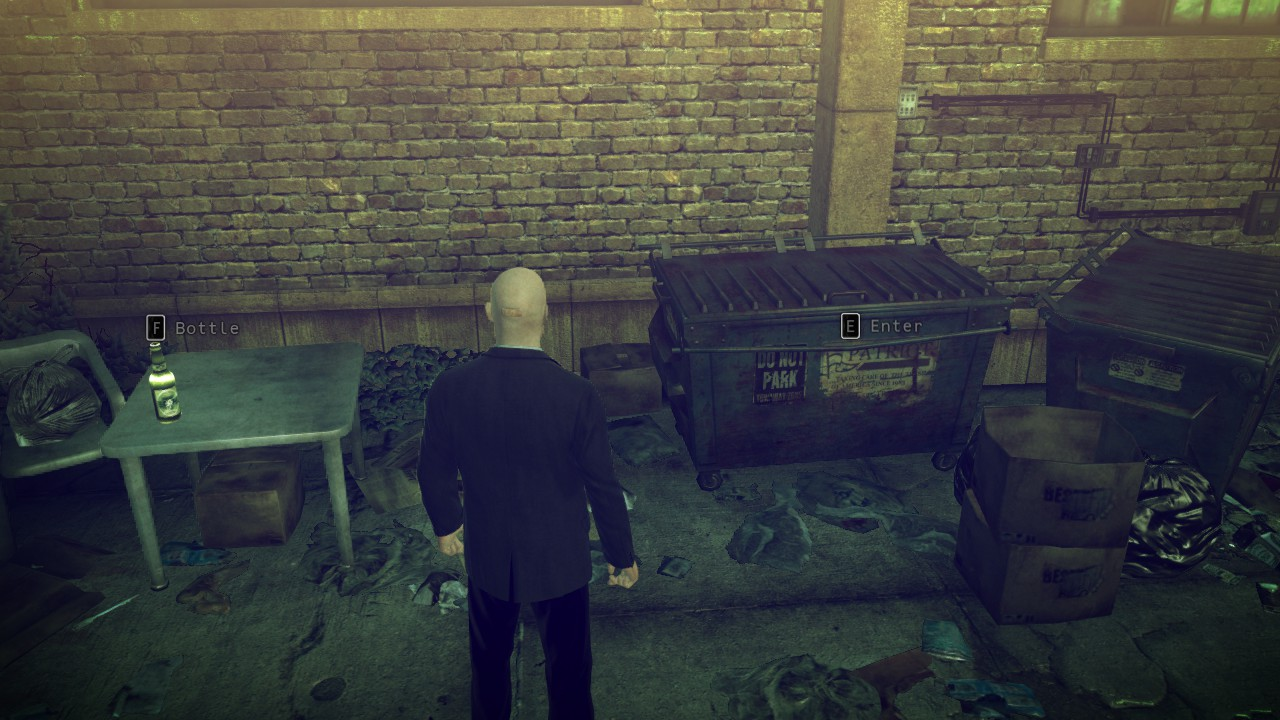
\includegraphics[width=11.5cm,keepaspectratio]{pics/shadows/ambientOcclusion/hitman}
  \end{figure}
\end{frame}

\begin{frame}\frametitle{Ambient occlusion}
  \begin{figure}[h]
    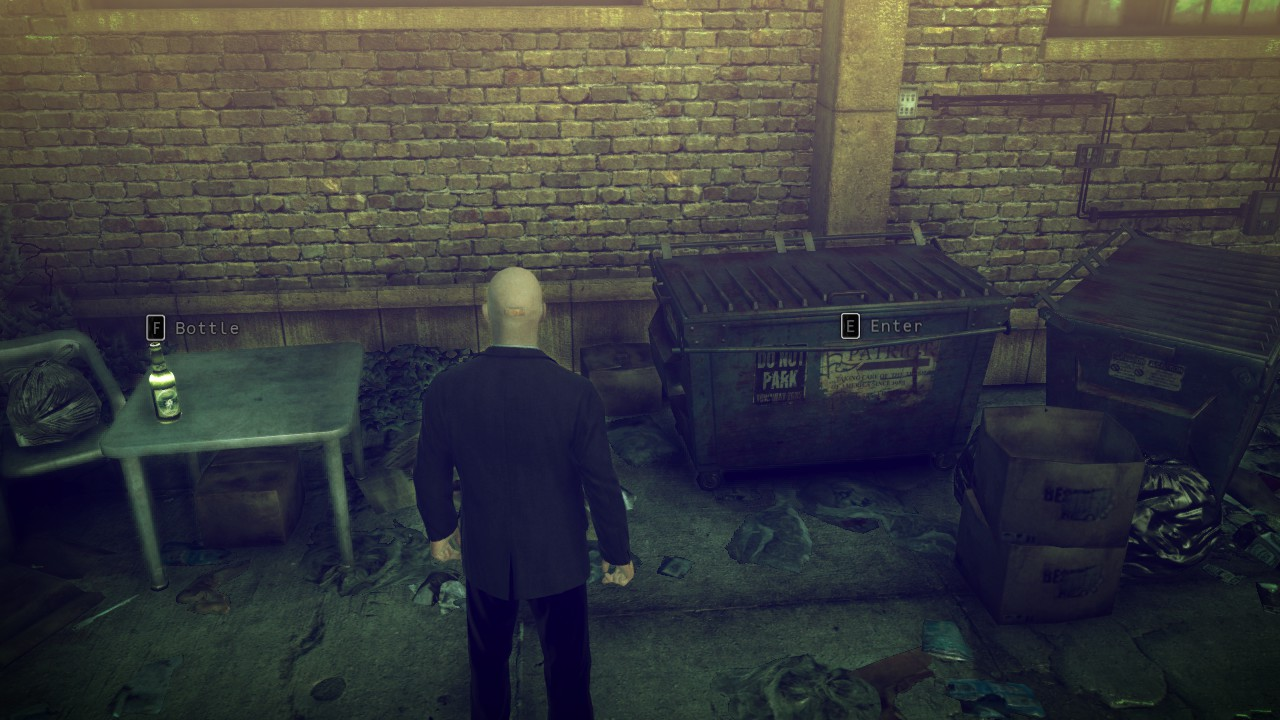
\includegraphics[width=11.5cm,keepaspectratio]{pics/shadows/ambientOcclusion/hitmanssao}
  \end{figure}
\end{frame}

\begin{frame}\frametitle{Ambient occlusion}
  \begin{figure}[h]
    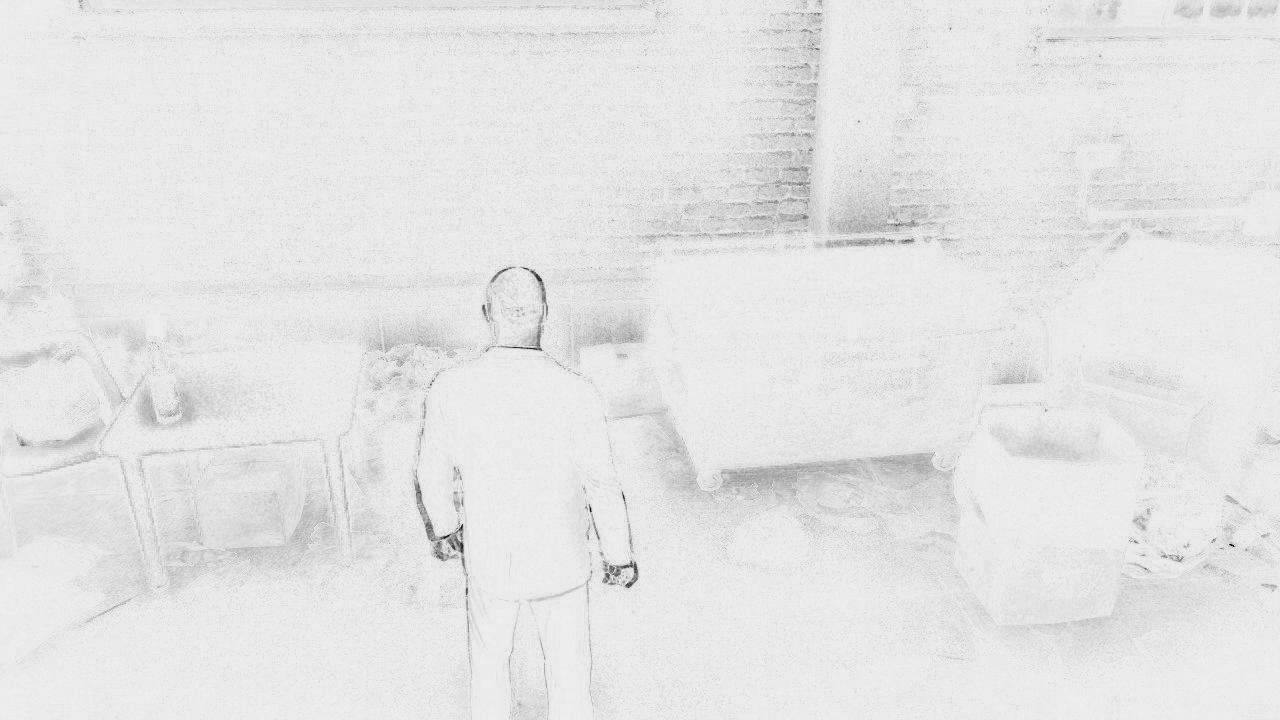
\includegraphics[width=11.5cm,keepaspectratio]{pics/shadows/ambientOcclusion/hitmanDifference}
  \end{figure}
\end{frame}
